\documentclass{cslthse-msc}
\setcounter{tocdepth}{4}
\setcounter{secnumdepth}{4}
\usepackage[utf8]{inputenc}
\usepackage[english]{babel}
\usepackage{amsmath}
\usepackage{amsfonts}
\usepackage{amssymb}
\usepackage{amsthm}
%\usepackage{makeidx}
\usepackage{graphicx}
\usepackage[titletoc, header, page]{appendix}
\usepackage{todo}
\usepackage{float}
\usepackage[hidelinks]{hyperref}
\usepackage{wrapfig}
\usepackage[within=none]{caption}
\usepackage{pdfpages}
\usepackage{svg}
\usepackage{listings}
\usepackage{color}
\newcommand{\hilight}[1]{\colorbox{yellow}{#1}}

\definecolor{mygreen}{rgb}{0,0.6,0}
\definecolor{mygray}{rgb}{0.5,0.5,0.5}
\definecolor{mymauve}{rgb}{0.58,0,0.82}


\lstset{
breaklines=true,
language=SQL,
numbers=left,
numbersep=5pt,
numberstyle=\tiny\color{mygray},
frame=single,
basicstyle=\footnotesize,
captionpos=b
}

\renewcommand{\lstlistingname}{Algorithm}% Listing -> Algorithm
\renewcommand{\lstlistlistingname}{List of \lstlistingname s}% List of Listings -> List of Algorithms



\author{
	Alexander Söderberg \\
	{\normalsize \href{mailto:email@alexandersoderberg.com}{\texttt{email@alexandersoderberg.com}}}
	\and
	Max Åberg \\
    {\normalsize \href{mailto:aaberg.max@gmail.com}{\texttt{aaberg.max@gmail.com}}}
}

\title{Optimizing business intelligence
extraction speed from an
ERP-system’s database}
\subtitle{Master Thesis}
\company{Perfect IT BeX\textsuperscript{\textregistered} AB}
\supervisors{Lennart Söderberg, \href{mailto:lennart@perfectit.se}{\texttt{lennart@perfectit.se}}}{Alma Orucevic Alagic, \href{mailto:alma@cs.lth.se}{\texttt{alma@cs.lth.se}}}
%\supervisor{John Deer, \href{mailto:jdeer@company.com}{\texttt{jdeer@company.com}}}
\examiner{Per Andersson, \href{mailto:per.andersson@cs.lth.se}{\texttt{per.andersson@cs.lth.se}}}

\date{\today}

\acknowledgements{
\todo{Skriv acknowledgments}
}

\theabstract{
\todo {Skriv abstract}

}

\keywords{MSc, MsSQL, ERP, Optimization}

%% Only used to display font sizes
\makeatletter
\newcommand\thefontsize[1]{{#1 \f@size pt\par}}
\makeatother
%%%%%%%%%%


\begin{document}
\makefrontmatter
\chapter[Introduction]{Introduction}
2014 was the year of the cloud. Software companies strived to make their services cloud based in order to meet the increasing demands from the market of availability and reliability. 
In today's businesses there's high demand for accurate and up-to-date business intelligence.

\chapter{Background}
\section{Background}

\section{Problem description}
\section{Thesis Goals}'


\section{Scope}
The time frame of a master thesis is limited and therefore work limitations have to exist. The system consists of several essential parts, all of which can be optimized in different extent. The focus of this thesis's is speed optimization of business intelligence reports and therefore the following limitations have been established:
\begin{itemize}
\item The optimization will not effect the systems front-end other than the speed of report generation.
\item The optimization will not effect the original structure of the systems database.
\item The optimization will not change the logic of the queries made by the back-end to the database.
\item The optimization should be versatile enough to handle future database expansions and higher performance of the system. However, in the scope of this master thesis only estimations based on the current system can be done.
\end{itemize}

\section{Related Work}
\section{Contributions}

\chapter{Research Questions \& Methodology}
\section{Research Questions}
\section{Methodology}
\section{Work}

\chapter{Approach}
\section{Technical System Description}
Perfect IT delivers web-based business system and services associated to such a market. All of the system components are essential parts of the business intelligence report generation, but only some of it are of interest when considering the extraction speed.
\begin{figure}[H]
\vspace{-15pt}
  \begin{center}
    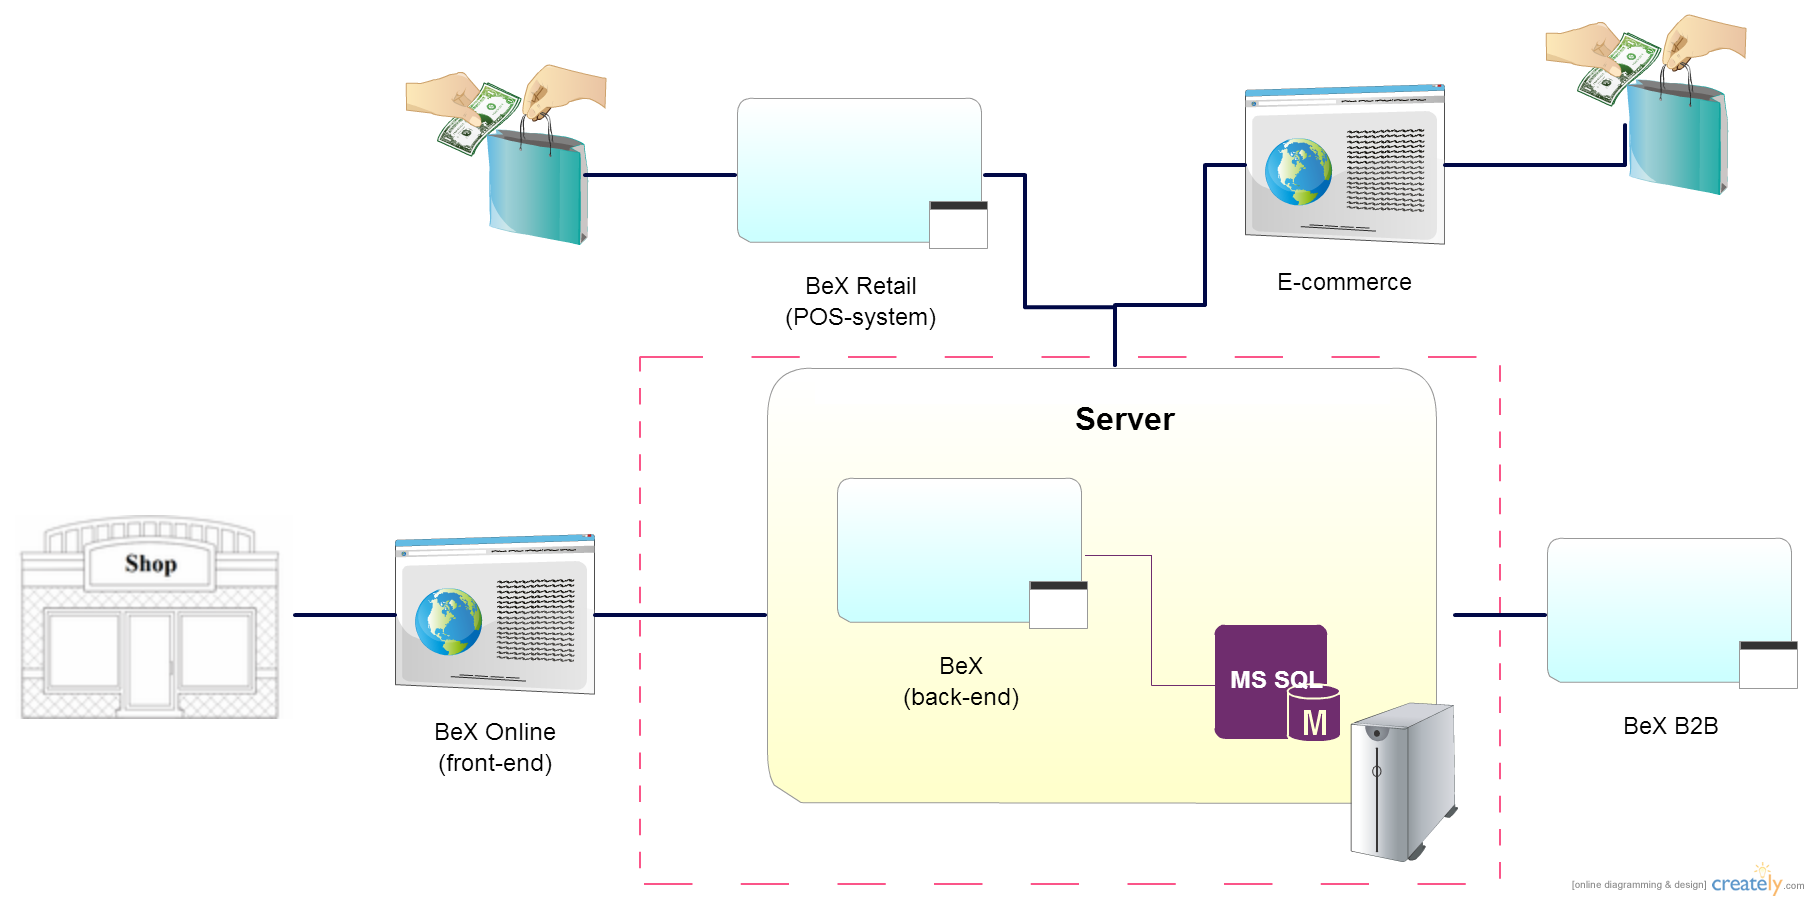
\includegraphics[scale=0.3]{Systemdesc.png}
  \end{center}
  \caption{Context diagram of Perfect IT's system}
  \label{context}
  \vspace{-15pt}
\end{figure}
\noindent The dashed section in Figure~\ref{context} are the components that are of the most interest for this thesis and will be more thoroughly described than the other system components.
\subsection{Components}
\subsubsection{BeX\textsuperscript{\textregistered} Online}
Each client possesses a unique instance of the BeX\textsuperscript{\textregistered} Online system, which consists of a front-end and a back-end a user interacts with. BeX\textsuperscript{\textregistered} Online is web based and has a front-end built in HTML5, CSS and JavaScript. The front-end communicates with the back-end through ASP (POST- \& GET-requests), which in turn translates the requests and sends SQL-queries to the database. The fetched result is finally interpreted by a web-browser as HTML. \todo{deeper description}
\subsubsection{Database}
The database is an essential part of Perfect IT's system and this thesis. All clients share the same physical database but have a unique instance of the database with only their data.  Perfect IT has has to today \hilight{40} clients connected to the servers database, all with different sizes of data ranging from approximately \hilight{5GB data to approximately 60GB} data. The database is run on an Microsoft SQL Server 2014 using OLTP and has a total of approximately \hilight{350GB} of data. The database design is largely the same for all the clients, with only a few exceptions among the clients.\\\\ 
This thesis will be using, until today, the biggest clients database measured in data. To ensure the clients privacy, all sensitive data has been encrypted by the system administrator. \\The default schema is called \textit{dbo} and consists of a total of 254 tables, including some views for big data queries. Many tables are large, considering the amount of rows, where the largest consists of approximately 10.5$\times 10^6$ rows. This table treats the data associated with every transaction made with the client from the start of using this system. There are also empty tables, \hilight{usage?}, that \ldots. The tables form a complex relation to each other and the references are many (as seen in this \href{https://drive.google.com/file/d/0B1IYTmE2hnD-eGQ0N2tvYXZNNVE/view?usp=sharing}{\textcolor{blue}{link}}). In the visualized database reference schema there are tables not referencing any tables at all, \hilight{why?}

\section{Theory}
In order to understand why a database might not perform optimally, the following theory was used.
\subsection{Index Fragmentation}
Index fragmentation is one of the most common problems in a relational database. Two kinds of fragmentation can occur, internal index fragmentation and external index fragmentation. The easiest way to explain index fragmentation is by imagining the SQL database as a phone book. At the very end of the book you have a few pages containing a table with indexes of all the entries sorted by last name. This is fine in a static environment such as a phone book but what happens in a dynamic environment?
Since people can be added to the phone book there must be space available after each column in the index, as well as in the pages in the phone book. This is called the \emph{fill factor}. A page can still run out of space and when this happens SQL Server has to add a new page, but it it can't add it at the correct place because the book is already bound. So, it adds blank pages at the very end. This causes two problems, pages with a lot of unused space and pages that are out of order. The first problem is what is referred to as \emph{Internal Fragmentation} and the second is \emph{External Fragmentation}. Internal fragmentation will of course also occur when deleting entries since that leaves "blank space" on the page.\cite{Ozar12}

\subsubsection*{Why is this bad for performance?}
At first, internal fragmentation might seem like a good thing. If the phone book has a lot of blank space on every page to start with, adding entries would be super easy and there would be no need for adding more pages later, causing external fragmentation. This is true, but when the number of extra pages needed in the phone book to allow for a lot of blank space is considered, the inefficiency of it becomes apparent. Going through a 100\% filled 1000 page phone book is much faster than a 90\% full 1100 page phone book. So in this example, every time SQL Server needs to scan the index, it would take 10\% longer. Another problem is that the lowest unit for caching in SQL Server is not a record, but a single page, which means that all the empty space must be cached as well. \\

External fragmentation often makes reading the database non-sequential, i.e it cannot be read in order but must be read in random order. This is especially bad in classic magnetic hard drives where the reader head must move around to multiple locations on the drive. Some magnetic hard drives only get 1\% of their sequential reading speed when performing random reads. \cite{Toshiba12}

\subsubsection*{Measuring fragmentation}
In Al-Farooque Shubho's article "Top 10 ways to optimize data access in SQL Server"\cite{Shubho09} he explains how to measure if index fragmentation has occurred. By executing the following script, index fragmentation is analyzed on every table in the database and presented in a table with an internal and external fragmentation value. 

\begin{lstlisting}[caption={Algorithm to find fragmented tables and the fragmentation values.},label=See DB-Fragmentation]
SELECT object_name(dt.object_id) Tablename,si.name
IndexName,dt.avg_fragmentation_in_percent AS
ExternalFragmentation,dt.avg_page_space_used_in_percent AS
InternalFragmentation
FROM
(
    SELECT object_id,index_id,avg_fragmentation_in_percent,avg_page_space_used_in_percent
    FROM sys.dm_db_index_physical_stats (db_id('AdventureWorks'),null,null,null,'DETAILED'
)
WHERE index_id <> 0) AS dt INNER JOIN sys.indexes si ON si.object_id=dt.object_id
AND si.index_id=dt.index_id AND dt.avg_fragmentation_in_percent>10
AND dt.avg_page_space_used_in_percent<75 ORDER BY avg_fragmentation_in_percent DESC
\end{lstlisting}

According to Shubho, only tables with an internal fragmentation value of less than 75 and/or an external fragmentation value of more than 10 should be considered as fragmented, which this code takes into account.

\subsubsection*{Reorganize vs. Rebuild}\mbox{}\\
Both rebuilding and reorganizing are built-in operations in SQL-Server 2014. These are two different operations that both reduce the fragmentation of the indexes. Reorganizing is the more lightweight of the two operations. It fixes the indexes as well as physical reordering of pages and applies any previously set fill factors. Rebuilding builds up a completely new structure for the index. It also allows for a new fill factor.\\
The advantage with reorganizing over rebuilding is that it can be aborted midway, while a rebuild must roll-back after an abort. Usually, in most SQL-systems, a rebuild can't be done while the SQL-server is online. This can be done in MS SQL Server Enterprise edition\cite{Little13}.

\subsubsection*{Is it always a good idea to fix fragmentation?}
According to Brent Ozar \cite{Ozar12} fixing fragmentation can cause more damage than keeping fragmented indexes. Often administrators try to fix fragmentation by using a low fill factor, say 50\%. This would mean that half of every page would be blank, which would make writing really fast. Reading however, would be twice as slow. Another common mistake is to rebuild every single index in the database, even though some tables might not had a single write since the last time. This is a problem because defragmenting indexes causes SQL Server to write to the transaction log. The bigger a log is, the longer log backups and restores take.\\

\subsection{Redundancy}

\subsection{Hekaton}

\section{Analysis}
\subsection{Index fragmentation}
By using the script from the theory the following index fragmentation values were produced.

\chapter{Proposed Solution}
\section{Solution Introduction}
\section{Integration}

\chapter{Software Development \& Testing}

\chapter{Discussion}

\chapter{Conclusions}
\addcontentsline{toc}{chapter}{Bibliography}
\bibliographystyle{plain}
\bibliography{MyMSc}
\begin{appendices}

\end{appendices}
\end{document}